
%Introduction
\section{Introduction}

In this report, we will discuss various points that must be decided before starting the implementation of the website. Those points are as follow : First, we will present the software architecture that we chose to use and extensively motivate this choice according to the project at hand. After that, we will once again motive our choice of framework but more extensively this time as it has to implement our architecture perfectly. Finally, we will present the current planned design of the website in the form of wireframes.

%Architecture
\section{Software architecture}
% Mainly Client & server architecture
% advantages for implementation and testing
% advantages for maintenance and evolution

The quality of the overall architecture of a software system is crucial to any project as it has to perfectly tailor to the need of that particular project. In fact, a good architecture would not only facilitate the implementation and testing of the software system but also its maintenance and evolutions.\newline

Great attention was thus given to the choice of a software architecture perfectly tailoring the need of our project and after extensively analysing the various architecture that exist, we settled on a 3-tier client-server architecture. \newline

\begin{figure}[H]
	\centering
	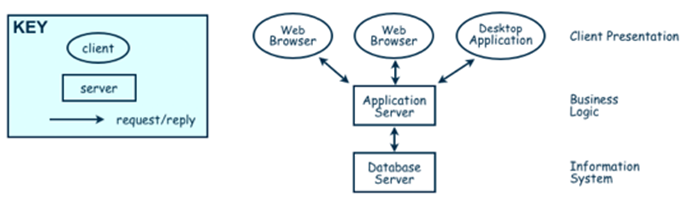
\includegraphics[width=0.9\linewidth]{ClientServerArchitecture.png}
	\caption{3-tier client-server architecture diagram}
	\label{fig:length_eight_mouse}
\end{figure}

This easily scalable architecture is perfectly tailored to the implementation of website in general as it allows multiple request to reach an application server without any loses. The transport of request/responses between the client browser and our server will be guaranteed by the http(s) protocol. \newline

The application server which process the various request of the clients will then acces/update the databases, following the need it faces. As this database connexion must be lossless to avoid critical errors, we will make use the TCP protocol to guarantee that everything comes through without losses. \newline

This allow for a simple yet scalable architecture that is highly evolutive. In fact, switching to a 4-tier or 5-tier architecture of the same model remains possible with minor change if the needs arise. Those n-tier architecture can contain additional layer proposing various utilities such as load balancing to redirect the traffic between application server or small additional servers that are tailored to process a certain part of the request. \newline

As you can see, this type of architecture is perfectly suited for this project as everything can be handled trough request, be it forms, searches or any other aspects of the program to code. This type architecture will also allow us to easily set up backup databases that would preserve the data in case of failure. \newline

In short this architecture will allow us to rapidly implement a working version of the project while using only the crucial component of the n-tier architecture. All while conserving the opportunity to easily scale up should the need arise. We believe that this scalable architecture will not only fulfil the current need of the clients for a working website but also their eventual future need in term scaling up their processing power to support more traffic.

%Frameworks
\section{Framework}

After having made our decision upon the software architecture, we must now choose which framework to use as to respect this architecture and ease the implementation of the website. In the three sections below, we detail the different frameworks that will be used to implement the various parts of the website and motive our choice of those specific frameworks. \newline

Of course, all frameworks that we even considered can be used to implement a 3-tier client-server architecture as they would be useless for us otherwise.

\subsection{Back-End}

The back-end handles everything related to the web server and the database. Using a framework will allow us to focus on the website development, without worrying too much about security, user management, administration panel, etc.\newline

After a long process of careful consideration and investigation, we decided on using \textbf{Django}, an open-source framework, for the back-end. It has a large community and is easy to learn. As a bonus, some group members already have some experience with this framework, making it easier for everybody to get started quickly.\newline

The main advantage of this framework being his architecture which is extremely well suited for implementing system based on a 3-tier client-server architecture (See figure 2). As you can see, \textbf{Django} relies on multiple layer of processes to handle request as swiftly and efficiently as possible. Each process having it's own role and being called only if necessary.  \newline

\begin{figure}
	\centering
	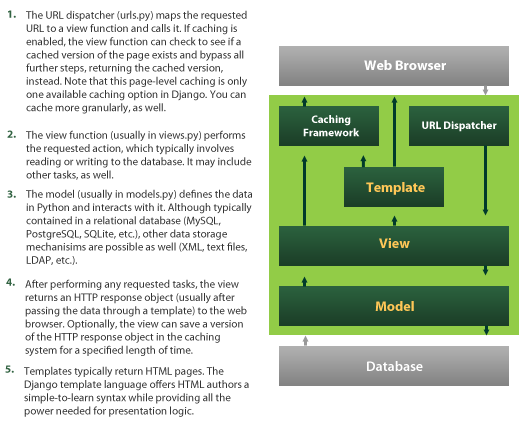
\includegraphics[width=0.85\linewidth]{DjangoArchitecture.png}
	\caption{Diagram of Django's architecture}
	\label{fig:length_eight_mouse}
\end{figure}

Another advantage of \textbf{Django} is the database management. \textbf{Django} uses Django-ORM which makes it really easy to communicate with the database. Django-ORM writes the SQL statements by itself. This allows us to use any type of database (sqLite, mySQL, PostgreSQL) and change it during the project development without impacting the rest of the project.
\textbf{Django} uses python as programming language. Python is easy to learn and, as we have to use it for our Artificial Intelligence course, learning it won't increase the work load at all.
Python is also very clean and easy to read thanks to its indentation syntax. Once again, multiple team members had experience with python, which is best to get started as quickly as possible.\newline

We also looked at the possibility of doing our website with \textbf{PHP}. Beside the fact that \textbf{PHP} is getting very old, it is still the most used back-end language on the web. But, its historical security problems and the fact that the code is included inside the HTML, are two important reasons that deterred us from choosing \textbf{PHP} for this project.\newline

\textbf{Ruby on rail} also seemed like a pretty good option and looked a lot like python, but none of our team members had experience with it, neither with the ruby language in general. Using Javascript was another option and some of our team member already used \textbf{NodeJS} in a previous project. But most of the people who had experience with this framework deterred us from using it again as they had a pretty bad experience with it (setting up the project may be long, there are a lot of different middle-wares to install to make your project run, community not always so helpful, ...).

\subsection{Front-End}

There are lots of tools to build a website design. The three main tools being HTML (creates the website elements), CSS (customizes elements with color, placement, and more) and JavaScript (used for validation, animation, forms, etc). Like for the back-end, there are frameworks built around those tools, making the work on the design easier, better, and faster. We will mainly use \textbf{Bootstrap}. It is a framework using HTML, CSS and JavaScript for developing responsive website for desktop and mobile. \textbf{Bootstrap} alone is not enough to build the whole website design. Another framework we are planning to use is \textbf{Angular JS}. It extends HTML with new attributes to handle events, forms, inputs, validations, and more. Allowing our website to be more efficient in general. \newline

With those two frameworks, we will be able to build most parts of the application. We might just need to add some more CSS to customize it if the need arise.

\subsection{Management}

We are using \textbf{Git} to have a private repository for our codes and reports of the project. We will also use \textbf{Trello}, a free web-based project management application using the Kanban paradigm. Both \textbf{Git} and \textbf{Trello} were used in the programming project of last year, so we all are quite familiar with these tools.

We will use Trello as a Kanban, and GitHub as a host for the code. \newline
